\documentclass[10pt]{article}
\usepackage{amsmath} 
\usepackage{fontspec}
\setmainfont{Arial}
\setmainfont[NFSSFamily=dayrom]{Arial}
\usepackage[a4paper, margin=12mm]{geometry}
\usepackage{graphicx}
\graphicspath{ {./images/} }

\usepackage{amsmath}

\DeclareSymbolFont{digits}{TU}{dayrom}{m}{n}
\AtBeginDocument{
	\DeclareMathSymbol{0}{\mathalpha}{digits}{`0}
	\DeclareMathSymbol{1}{\mathalpha}{digits}{`1}
	\DeclareMathSymbol{2}{\mathalpha}{digits}{`2}
	\DeclareMathSymbol{3}{\mathalpha}{digits}{`3}
	\DeclareMathSymbol{4}{\mathalpha}{digits}{`4}
	\DeclareMathSymbol{5}{\mathalpha}{digits}{`5}
	\DeclareMathSymbol{6}{\mathalpha}{digits}{`6}
	\DeclareMathSymbol{7}{\mathalpha}{digits}{`7}
	\DeclareMathSymbol{8}{\mathalpha}{digits}{`8}
	\DeclareMathSymbol{9}{\mathalpha}{digits}{`9}
}

% Footer-Einstellungen
\usepackage{fancyhdr}
\usepackage{amsmath}
\usepackage{datetime}
\newdateformat{mydate}{\twodigit{\THEDAY}.\twodigit{\THEMONTH}.\THEYEAR}
\mydate
\pagestyle{fancy}
\fancyhf{} % Löscht alle Kopf- und Fusszeilen
\fancyfoot[C]{\thepage\ -\ \today\ \copyright\ Bastian\ Kind,\ James\ Binks,\ Mark\ Matkovic\ und\ David\ Hafner} % Setzt den Footer

\title{DFB Entdecker App}
\author{Bastian Kind, James Binks, Mark Matkovic und David Hafner}

\begin{document}
	\maketitle
	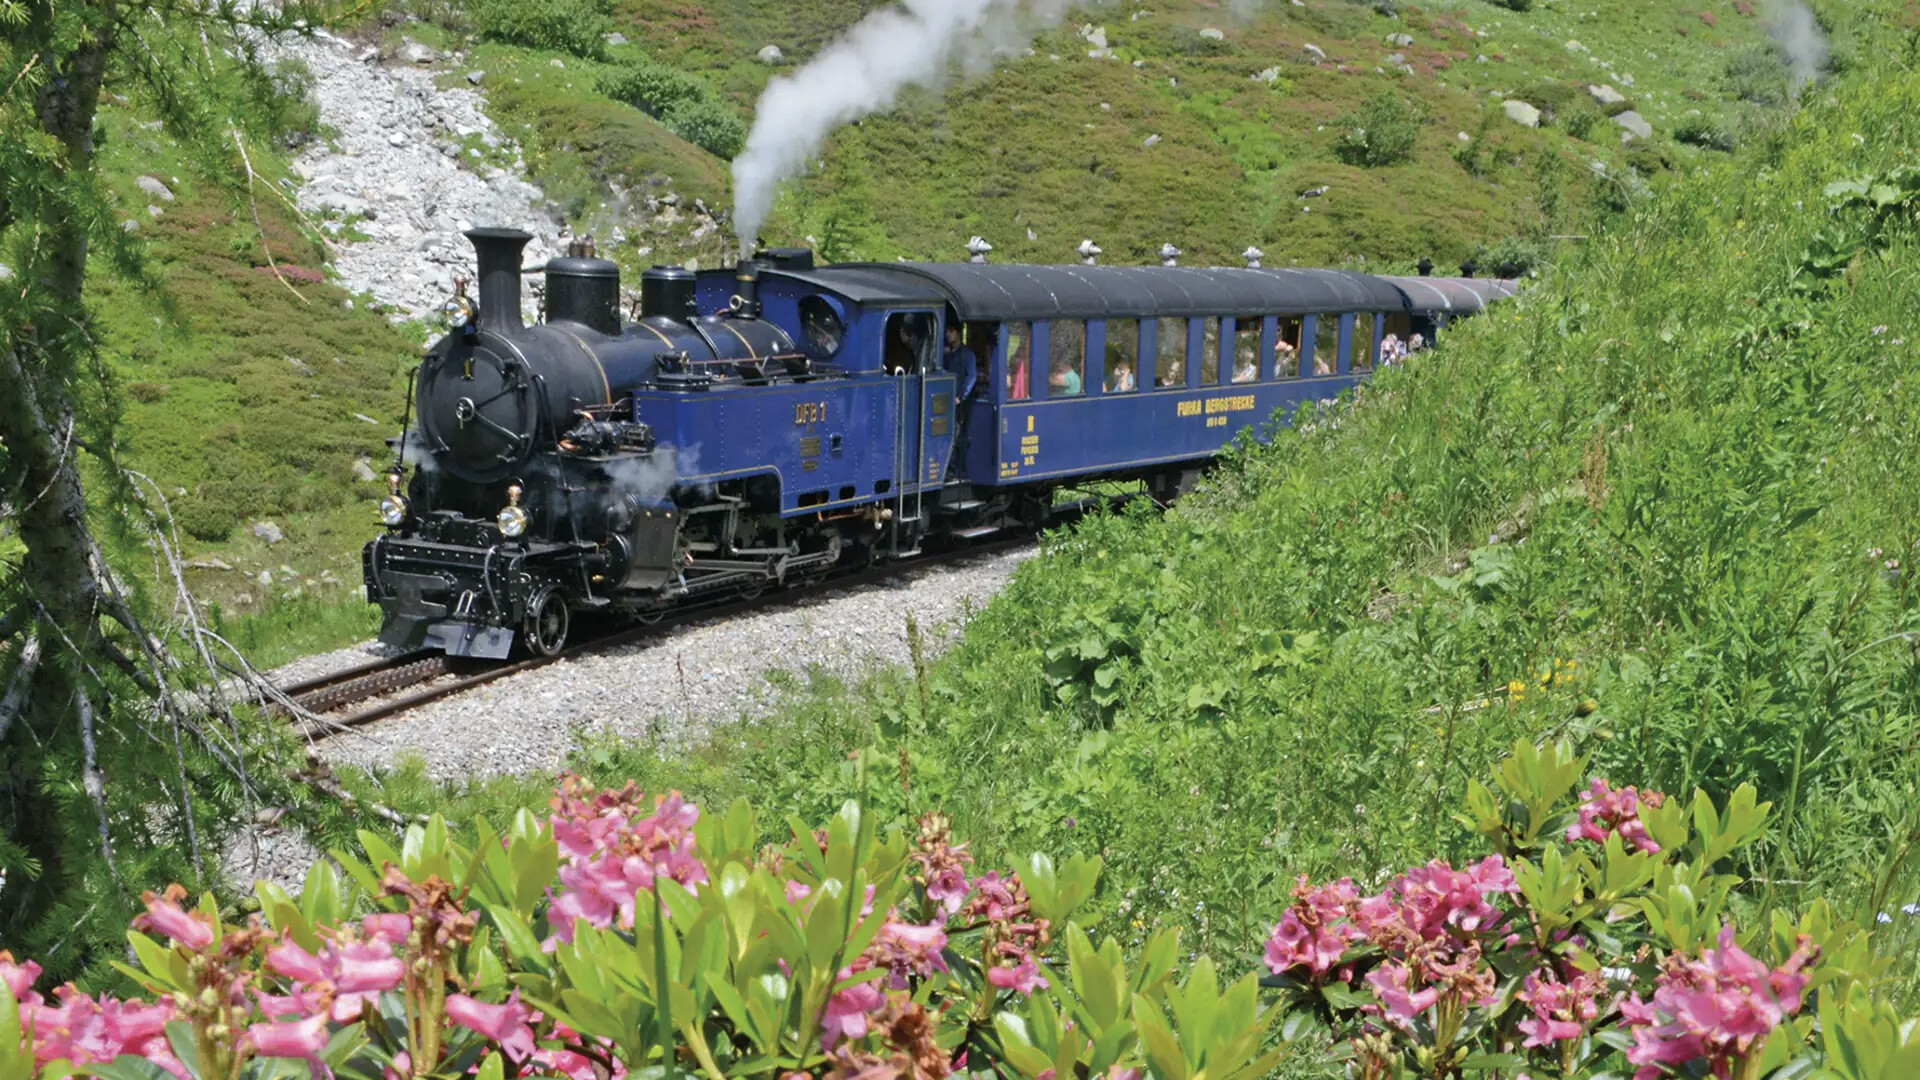
\includegraphics[width=17.5cm]{title}
	\pagebreak
	\tableofcontents
	\pagebreak
	\section{Band A}
	\subsection{Anforderungsanalyse}
	\subsubsection[Wer]{Wer benutzt die App?}
	\begin{itemize}
		\item Familien mit Kindern (z.\,B. als Freizeit-Ausflug)
		\item Rentner / ältere Menschen (Interesse an Geschichte und Eisenbahn)
		\item Erwachsene allgemein (z.\,B. Eisenbahnbegeisterte, Touristen)
		\item Schulklassen (für interaktive, spielerische Lernmöglichkeiten)
	\end{itemize}
	\subsubsection[Wo]{Wo wird die App verwendet?}
	\begin{itemize}
		\item Entlang der Furka-Bergstrecke, einer historischen Dampfbahnstrecke
		\item Draussen (z.B. auf Bahnhöfen, an Brücken, bei Aussichtspunkten)
		\item Oft ohne Mobilfunknetz -> App muss offlinefähig sein
		\item Unterwegs mit dem Zug oder zu Fuss an Haltepunkten
	\end{itemize}
	\subsubsection[Was]{Was muss die App können?}
	\begin{itemize}
		\item QR-Codes an Infopunkten scannen -> Inhalte anzeigen (Text, Bilder, Videos, Audio)
		\item Karte mit GPS nutzen -> aktuelle Position und nahegelegene Punkte anzeigen
		\item Quiz- oder Rätsel-Funktion -> spielerisches Lernen
		\item Tagebuch- oder Sammelfunktion («Meine liebsten Sehenswürdigkeiten»)
		\item Inhalte in mehreren Sprachen (D/E/F/I), evtl. auch einfache Sprache
		\item Inhalte offline verfügbar
		\item Datenschutzkonform -> keine Registrierung, keine Standortüberwachung / Standort wird nicht gespeichert
	\end{itemize}
	\subsubsection[Womit]{Technische Rahmenbedingungen}
	\begin{itemize}
		\item Smartphone oder Tablet, Android und iOS (Dynamisch)
		\item Ressourcenschonendes Design (damit es auch auf älteren Geräten läuft)
		\item App soll Inhalte aus CMS (z.\,B. Texte, Medien) beziehen
		\item Kein Internet nötig unterwegs (alle Inhalte offline verfügbar)
		\item Barrierefreiheit: Vorlesefunktion, grosse Schrift, starke Kontraste
	\end{itemize}
	\subsubsection[Verbesserungen]{Verbesserungen}
		\begin{itemize}
			\item Wir könnten die Benutzergruppen noch genauer unterteilen. Z.\,B. nach technischen Kentnissen, Alter oder ob die Nutzer einheimische oder Touristen sind.
			\item Wir könnten konkrete Anforderungen für barrierefreies Design formulieren. Z.\,B. Schriftgrössen, Bedienung mit Screenreader, Kontraste
			\item Wir könnten die Datenschutzanforderungen genauer definieren. Z.\,B. Wie werden die GPS Daten verarbeitet?
			%\item \textbf{Gamification weiterdenken:} Die Rätsel- und Sammelfunktionen könnten mit Badges, Levels oder Belohnungen erweitert werden, um die Motivation zu steigern.
		\end{itemize}
		\pagebreak
	\subsection{Vorgehensmodell}
		\subsubsection{Wahl des Modells}
		% Erklärung, welches Vorgehensmodell gewählt wurde (z. B. Design Thinking, User Centered Design) und warum
		Wir haben das Vorgehensmodell Design Thinking gewählt, da es gut zu unserem Projekt passt. Es ist benutzerorientiert und iterativ. Es gibt viel Nutzerfeedback und das Endprodukt ist das, was der Nutzer will.\\
		So können wir sicherstellen, dass wir uns nicht in Details verlieren, die dem Nutzer schlussendlich wenig nützen. Wir werden uns so besser auf die Wünsche und die Bedürfnisse des Nutzers konzentrieren können.
		\subsubsection{Phasen des Modells}
		% Beschreibung der einzelnen Phasen des gewählten Modells mit kurzer Erklärung (z. B. beim Design Thinking: Verstehen, Beobachten, Sichtweise definieren, Ideen finden, Prototyp bauen, Testen)
		Design Thinking hat zwei «Räume». Es gibt den Problemraum und den Lösungsraum. Im Problemraum schaut man die Probleme an.
		\begin{itemize}
			\item Verstehen
			\subitem Als erstes muss man das Umfeld und die Nutzer verstehen.
			\item Beobachten
			\subitem Dann schaut man, wie sich der Nutzer verhält.
			\subitem Was macht der Nutzer, was ist ihm am wichtigsten, womit verbringt er viel Zeit.
			\item Standpunkt definieren
			\subitem Die gewonnen Erkenntnisse muss man dann aufschreiben und nach Wichtigkeit filtern oder sortieren.
			\subitem Möglicherweise braucht man noch mehr Informationen und muss nochmals zu einem der beiden vorherigen Schritte zurückgehen.
		\end{itemize}
		Im Lösungsraum überlegt man sich dann Lösungen für die gefundenen Probleme.
		\begin{itemize}
			\item Ideen finden
			\subitem Im ersten Schritt im Lösungsraum überlegt man sich, wie man die Probleme lösen könnte
			\item Prototyp entwickeln
			\subitem Zu diesen Ideen entwickelt man dann einen Prototypen.
			\item Testen
			\subitem Diesen Prototypen testet man dann mit dem Nutzer
			\subitem Mit dem erhaltenen Feedback muss man dann evtl. Zu einem der vorherigen Schritte zurückkeren und Verbesserungen vornehmen.	
		\end{itemize}
		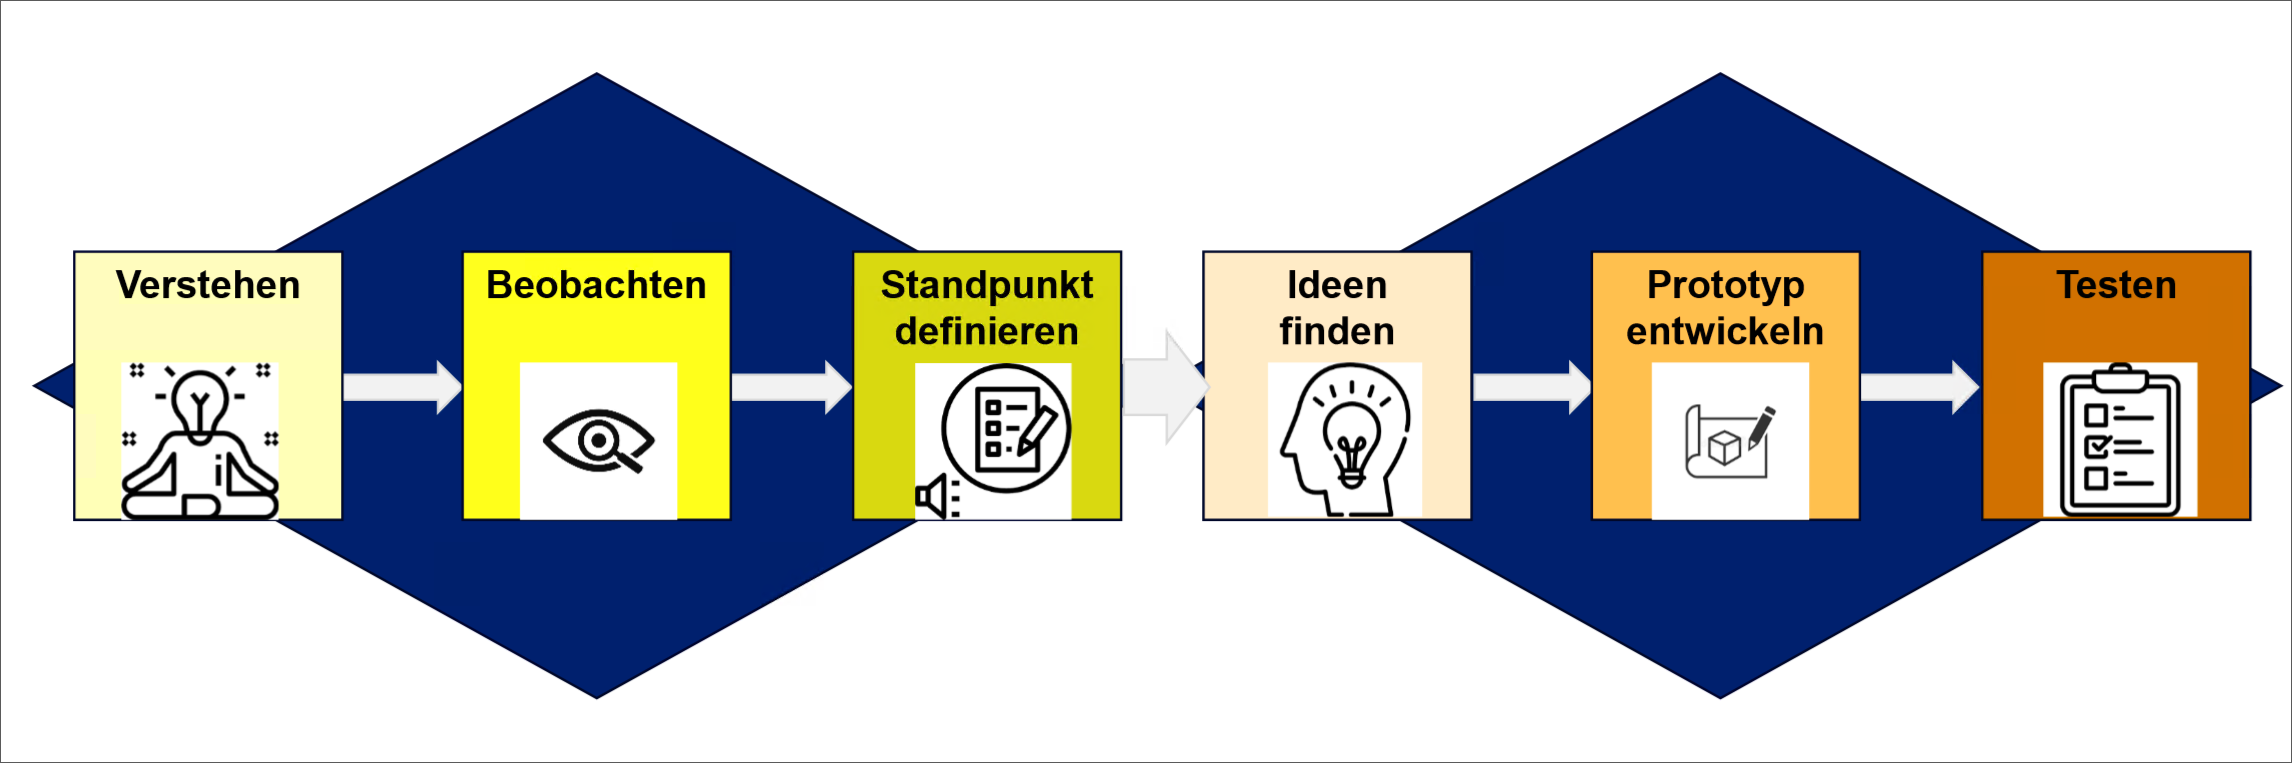
\includegraphics[width=18.6cm]{DesignThinking}
	\pagebreak
	\subsection{Nutzungskontext}

\subsubsection{Methoden zur Kontextanalyse}

\begin{itemize}
	\item Beobachtungen vor Ort entlang der Strecke
	\item Interviews mit Besuchern
	\item Analyse von Bewertungen der DFB
	\item Elektronische Umfragen
\end{itemize}

\subsubsection{Analyseergebnisse}
\begin{itemize}
	\item Die Strecke liegt in einem abgelegenen Berggebiet – Mobilfunknetz ist nur teilweise verfügbar.
	\item Die Nutzung erfolgt draussen: an Bahnhöfen, Aussichtspunkten, Infotafeln oder im Zug.
	\item Nutzer sind häufig zu Fuss unterwegs und haben nur kurz Zeit für Interaktion.
	\item Zielgruppe ist sehr durchmischt: Kinder, Erwachsene, Senioren, Touristen, Schulklassen.
	\item Viele Nutzer wünschen sich eine spielerische, leicht verständliche und multilinguale Erfahrung. (Viedos und illustration)
\end{itemize}

\subsubsection{Schlussfolgerungen für die App}
\begin{itemize}
	\item Die App muss vollständig offlinefähig sein.
	\item Eine einfache Bedienung ist nötig, besonders für Kinder und ältere Menschen.
	\item Ein intuitives und zweckdienliches Design
	\item Barrierefreiheit ist wichtig: grosse Schrift, kontrastreiche Farben, Vorlesefunktion.
	\item Inhalte müssen mehrsprachig verfügbar sein (De/En/Fr/It), mit vereinfachtem Deutsch für Kinder.
	\item Zusätzliche detailliertere informationen für enthusiasten.
	\item Die App sollte schnell Informationen liefern, da Nutzer meist unterwegs oder in Bewegung sind.
\end{itemize}
\pagebreak
\subsection{Benutzereigenschaften}
\subsubsection{Warum werden Benutzereigenschaften erfasst}
\begin{itemize}
	\item Wir erfassen Benutzereigenschaften, damit wir uns besser vorstellen können, welche Bedürfnisse die Benutzer haben und wie sie sich verhalten.
	\item Wenn wir die Ziele der Benutzer erfassen, also was die Benutzer auf der App wollen, können wir schauen, dass sie ihre Ziele einfacher erreichen können.\
	\item Die Benutzerbedürfnisse erfassen wir, damit wir diese in den Vordergrund stellen können. So priorisieren wir das, was den Nutzern am wichtigsten ist.
\end{itemize}
\subsubsection{Personas}
\begin{itemize}
	\item \textbf{Familie Müller} (Eltern 40/38, Kinder 8/12)
	\subitem \textbf{Hintergrund}: Tagesausflug mit Kindern, wenig technikaffin
	\subitem \textbf{Ziele}: 
	\begin{itemize}
		\item Schneller Zugang zu kindgerechten Inhalten
		\item Offline-Karten für Wanderwege
		\item Spielerische Quiz-Funktion
	\end{itemize}
	\subitem \textbf{Schmerzpunkte}: 
	\begin{itemize}
		\item Komplexe Menüs
		\item Lange Ladezeiten ohne Netz
	\end{itemize}
	
	\item \textbf{Hans Meier} (65, Eisenbahn-Enthusiast)
	\subitem \textbf{Hintergrund}: Pensioniert, historisch interessiert
	\subitem \textbf{Ziele}: 
	\begin{itemize}
		\item Technische Details zu Lokomotiven
		\item Historische Vergleichsbilder
		\item Präzise GPS-Positionsanzeige
	\end{itemize}
	\subitem \textbf{Schmerzpunkte}: 
	\begin{itemize}
		\item Kleine Schriftgrössen
		\item Fehlende Tiefeninformationen
	\end{itemize}
	
	\item \textbf{Laura Bianchi} (28, internationale Touristin)
	\subitem \textbf{Hintergrund}: Backpacking in der Schweiz
	\subitem \textbf{Ziele}: 
	\begin{itemize}
		\item Mehrsprachige Audio-Guides (EN/IT)
		\item Social-Media-Integration
		\item Datensparsame Nutzung
	\end{itemize}
	\subitem \textbf{Schmerzpunkte}: 
	\begin{itemize}
		\item Hoher Datenverbrauch
		\item Unklare Wegführung
	\end{itemize}
	
	\item \textbf{Teenager Alex} (15, lokaler Jugendlicher)
	\subitem \textbf{Hintergrund}: Nutzt App mit Schulkameraden
	\subitem \textbf{Ziele}: 
	\begin{itemize}
		\item Gamification (Badges sammeln)
		\item Foto-Challenges mit Hashtags
		\item Schnelles Teilen von Entdeckungen
	\end{itemize}
	\subitem \textbf{Design-Implikation}: 
	\begin{itemize}
		\item Einfache Social-Media-Buttons
		\item Visuell ansprechende Achievements
	\end{itemize}
\end{itemize}
\subsubsection{Verbesserungen}
\begin{itemize}
	\item \textbf{Familie Müller (Kinder-Modus)}
	\subitem \textbf{Problem}: 
	\begin{itemize}
		\item Quiz-Fragen nicht altersgerecht differenziert
		\item Eltern/Kinder nutzen dieselbe Oberfläche
	\end{itemize}
	\subitem \textbf{Anpassung}: 
	\begin{itemize}
		\item „Kinder-Modus“ mit vereinfachten Fragen + Emojis
		\item Eltern können Modus per Passcode sperren
	\end{itemize}
	\subitem \textbf{Design-Implikation}: 
	\begin{itemize}
		\item Toggle-Schalter „Kindermodus“ in der Navigation
		\item Visuelle Icons statt Textbuttons
	\end{itemize}
	
	\item \textbf{Hans Meier (Schriftgrösse)}
	\subitem \textbf{Problem}: 
	\begin{itemize}
		\item Standard-Schrift für Outdoor-Nutzung zu klein
		\item Keine Anpassungsmöglichkeiten
	\end{itemize}
	\subitem \textbf{Anpassung}: 
	\begin{itemize}
		\item Schriftgrössen-Slider (100\%–200\%)
		\item Kontrastmodus für Sonnenlicht
	\end{itemize}
	\subitem \textbf{Design-Implikation}: 
	\begin{itemize}
		\item Dynamische UI-Anpassung aller Textelemente
		\item Persistente Einstellung über App-Neustart
	\end{itemize}
	
	\item \textbf{Laura Bianchi (Sprachumschaltung)}
	\subitem \textbf{Problem}: 
	\begin{itemize}
		\item Sprachwechsel erfordert 4 Klicks
		\item Keine Gerätesprachen-Erkennung
	\end{itemize}
	\subitem \textbf{Anpassung}: 
	\begin{itemize}
		\item Automatische Sprachwahl basierend auf Gerät
		\item Sprach-Icon in Top-Leiste
	\end{itemize}
	\subitem \textbf{Design-Implikation}: 
	\begin{itemize}
		\item Dropdown-Menü mit Flaggen-Icons
		\item Sprachwechsel ohne App-Neustart
	\end{itemize}
	
	\item \textbf{Teenager Alex (Gamification)}
	\subitem \textbf{Problem}: 
	\begin{itemize}
		\item Achievements motivieren nicht nachhaltig
		\item Keine Social-Media-Verlinkung
	\end{itemize}
	\subitem \textbf{Anpassung}: 
	\begin{itemize}
		\item „Badge-System“ mit Leveln (Bronze–Platin)
		\item Direktes Teilen auf Instagram/TikTok
	\end{itemize}
	\subitem \textbf{Design-Implikation}: 
	\begin{itemize}
		\item Progress-Bar im Profil-Bereich
		\item Ein-Klick-Share-Buttons
	\end{itemize}
\end{itemize}

\subsubsection{Priorisierung der Anpassungen}
\begin{center}
	\begin{tabular}{|l|l|l|}
		\hline
		\textbf{Anpassung} & \textbf{Relevanz} & \textbf{Aufwand} \\ 
		\hline
		Schriftgrössen-Slider & Hoch & Niedrig \\
		Kinder-Modus & Mittel & Mittel \\
		Automatische Sprachwahl & Hoch & Hoch \\
		Badge-System & Mittel & Hoch \\
		\hline
	\end{tabular}
\end{center}

\textit{Begründung: Schriftgrössen-Slider wurde priorisiert, da essenziell für Barrierefreiheit und einfach umsetzbar.}
\pagebreak
\subsection{Nutzungsanforderungen}
\subsubsection{Einleitung}
Die Spezifikation der Nutzungsanforderungen ermöglicht es, die Bedürfnisse der Nutzer in konkrete To-Dos umzuwandeln.\\
Dafür verwenden wir User Stories, die typische Nutzungssituationen beschreiben.
\subsubsection{User Stories}
\begin{itemize}
	\item Als Familienvater möchte ich eine Simple und intuitive Darstellung, so dass meine Kinder alles verstehen können.
	\item Ich als Senior möchte eine Grosse und klare Schrift, so dass ich diese gut lesen kann.
	\item Als Tourist möchte ich eine Karte mit GPS-Ortung nutzen können, um interessante Punkte entlang der Strecke zu finden.
	\item Als Kind möchte ich Quizfragen beantworten, damit ich spielerisch etwas über die Eisenbahn lernen kann.
	\item Als Lehrperson möchte ich die App offline nutzen können, damit ich mit der Klasse auch ohne Netz arbeiten kann.
\end{itemize}

\subsubsection{Priorisierung}
\begin{itemize}
	\item \textbf{Must-Have}: QR-Scan, Offline-Funktion, mehrsprachige Inhalte, intuitive Bedienung
	\item \textbf{Should-Have}: Quizfunktion, GPS-Karte, Tagebuch/Sammelmodus
	\item \textbf{Could-Have}: Dialekte, individuelle Empfehlungen, erweiterte Suchfunktion
\end{itemize}
\end{document}